% 2008 年四川卷理科第 21 题：椭圆左、右焦点 F1、F2，离心率 √2/2，右准线 l，
%   M、N 为 l 上的两个动点，F1M · F2N = 0。
% 来源 PDF：gaokaomath-src/普通高考/2008/2008四川理.pdf
% SHA-256：dd251cfc43d7be2f75e2675f8bd73e8569900c65a53724312a95b1cec79a3a9b
% 原页：2008四川理.pdf 第 2 页（A3 三栏）第 2 栏，书页码 484。
% 绘制依据：按原页画 x/y 轴与 O、椭圆、F1/F2，右准线 l 为竖直线，M 在 l 上方、N 在 l 下方，
%   F1—M 与 F2—N 为实线并互相垂直。
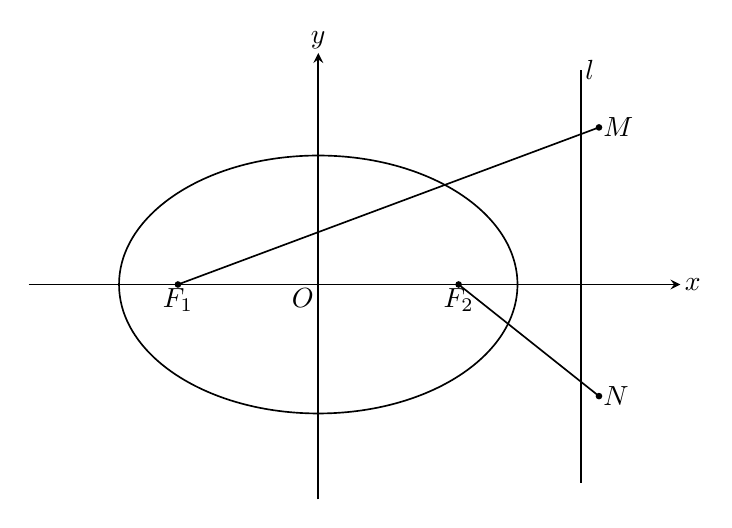
\begin{tikzpicture}[x=1.15cm, y=1.05cm, semithick, every node/.style={inner sep=1.3pt}]
  \draw[->,>=stealth] (-3.2,0) -- (4.0,0) node[right] {$x$};
  \draw[->,>=stealth] (0,-2.6) -- (0,2.8) node[above] {$y$};
  \node[below left] at (0,0) {$O$};

  \draw (0,0) ellipse [x radius=2.2, y radius=1.56];

  \coordinate (F1) at (-1.55,0);
  \coordinate (F2) at (1.55,0);
  \coordinate (M) at (3.1,1.9);
  \coordinate (N) at (3.1,-1.35);

  \draw (2.9,-2.4) -- (2.9,2.6);
  \node[right] at (2.9,2.6) {$l$};

  \draw (F1) -- (M);
  \draw (F2) -- (N);

  \fill (F1) circle (1.2pt); \node[below] at (F1) {$F_1$};
  \fill (F2) circle (1.2pt); \node[below] at (F2) {$F_2$};
  \fill (M) circle (1.2pt); \node[right] at (M) {$M$};
  \fill (N) circle (1.2pt); \node[right] at (N) {$N$};
\end{tikzpicture}
